\documentclass[10pt]{article}

\def\Type{LessonCaelan}
\def\TypeNum{Lesson 14}
\def\TypeTitle{Applied Optimization\\Solutions }
\def\Semester{Fall 2021} %Not Used 
\def\Course{MATH 1190 \& 1210}
\def\Targets{  {\bf\color{RedOrange}A3} }

\usepackage{preambleDJ}


%%%%%%%%%%%% BEGIN DOCUMENT %%%%%%%%%%%%%%%
%%%%%%%%%%%% BEGIN DOCUMENT %%%%%%%%%%%%%%%
%%%%%%%%%%%% BEGIN DOCUMENT %%%%%%%%%%%%%%%
%%%%%%%%%%%% BEGIN DOCUMENT %%%%%%%%%%%%%%%
%%%%%%%%%%%% BEGIN DOCUMENT %%%%%%%%%%%%%%%




\begin{document}

\pagestyle{otherpages}
\thispagestyle{firstpage}
\vs{.65}
{\bf\color{blue}Read the Passage.} In the online pre-class activity, we saw optimization problems solved in two phases: the modeling phase and the calculus phase. We'll practice specific steps within each of those phases in this activity while re-attempting some of the same problems that appeared in the pre-class assignment - as well as while trying new problems.\\

Try to work through the following problem, which appeared in the pre-class assignment (with different numbers) as example 1. You don't have to get everything right - that you are willing to try something, figure out a method, and make some mistakes along the way is far more important than feeling pressured to get everything right the very first time.\\

{\bf\color{blue}Warm-up exercise 1.}\ltrm{\bf\color{RedOrange}A3} We want to build an open box (four side walls and a bottom but no top) with a square base. The volume of the box must be $256$ cm$^3$. We should build the box to spend as little on the materials as possible. What dimensions should we choose for our box?\\

\textbf{Modelling Phase:}\\
\mpageTth{.3}{.4}{.4}{
 \graphicsL{box}{2}
}{
$$SA=Bottom_{area}+Sides_{area}$$
\sol{
\itemI{
\item The bottom of the box is a square so $Bottom_{area}=side\times side=x\cdot x=x^2$
\item The sides of the box are rectangles and there are $4$ sides, so \\$Sides_{area}=4\times width\times height = 4\cdot x\cdot y$
\item Thus the surface area is $$SA=Bottom_{area}+Sides_{area}=x^2+4xy$$
}
}
}{
$$V=Length \times Width \times Height$$
\sol{
\itemI{
\item The bottom of the box is a square, so Length and width are the same:\\ $L=W=x$
\item Height is represented by the variable $y$
\item We are told volume is $256$ cm$^3$
\al{
V&=Length \times Width \times Height\\
256&= x\cdot x\cdot y\\
256&=x^2y
}
}
}
}
\blue{
 The goal of this question is to find the absolute minimum of the surface area of the box.  The challenge  is that $SA=x^2+4xy$ is a function of two variables ($x$ and $y$), and we need a function of one variable in order to  find absolute minimum. So we utilize our constraint involving the volume and solve for one variable (it doesn't matter which variable you solve for).
$$\ds 256=x^2y \Rightarrow y=\frac{256}{x^2}$$
We utilize this in our surface area equation:
\al{
SA&=x^2+4xy\\
SA&=x^2+4x\left( \frac{256}{x^2}\right)\\
SA&=x^2+4\left( \frac{256}{x^1}\right) \\
SA&=x^2+1024x^{-1} \\
}
We further assume that since $x$ is a length, it must be positive. Therefore the domain is $x>0$ or $(0,\infty)$
}
\newpage
\textbf{Calculus Phase:}
\sol{
We find the absolute maximum 
\enum{
\item Find critical numbers. We check when $SA^{\prime}(x)=0$ and if $SA^{\prime}(x)\;DNE$\\
\mpageT{.5}{.5}{
When does $SA^{\prime}(x)=0$?
\al{
SA(x)&=x^2+1024x^{-1}\\
SA^{\prime}(x)&=2x-1024 x^{-2}\\
0&\stackrel{??}{=} 2x-\frac{1024}{x^2}\\
\frac{1024}{x^2} &  \stackrel{??}{=}2x\\
\frac{1024}{2} &\stackrel{??}{=}x^3\\
512 &\stackrel{??}{=}x^3\\
\sqrt[3]{512}&\stackrel{??}{=} x\\
8&=x
}
}{
When does $SA^{\prime}(x)=DNE$?\\
Since $\ds SA^{\prime}(x)=2x+\frac{1024}{x^2}$, we have a division by $0$ when $x=0$.\\\\ Thus $\ds SA^{\prime}(0)\;DNE$.\\\\
But $x=0$ is not in the domain of $(0,\infty)$ so it is not a critical number. 
}
Since we have only one critical number in the domain, we hope to use the First Derivative Test for Absolute Extrema from last class. In order to do that, we must set up a sign line.  \\
\mpageT{.7}{.4}{
\itemI{
\item Choose  value in $(0,8)$, say $x=1$. $\ds SA^{\prime}(1)=2\cdot 1-\frac{1024}{1^2}=-1022$
\item Choose  value in $(8,\infty)$, say $x=10$. $\ds SA^{\prime}(10)=2\cdot 10-\frac{1024}{10^2}=9.76$
}
}{
\begin{center}
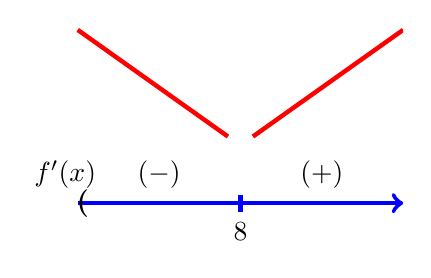
\begin{tikzpicture}
 \begin{axis}[
    	axis x line=none,
	            axis y line=none,
		x label style={anchor=west},
            xlabel={},
            xtick       = {8},
            xticklabels = {$8$},
            y label style={anchor=south},
            ylabel={},
            ytick       = {-6,-4,-2,2,4,6},
            yticklabels = {$-6$,$-4$,$-2$,$2$,$4$,$6$},
            samples     = 320,
            domain      = -2.5:2.5,
            restrict y to domain=-6.5:6.5,
            xmin = 0, xmax = 15,
            ymin = -6.5, ymax = 6.5,
            width=2.5in, height=2.5in,
            grid=none, grid style=solid
          ]
    \addplot[domain= 2:15, blue, ultra thick, mark=none, ->]{0)};
        \addplot[domain= 2:8, red, ultra thick, mark=none, -]{-4/6.5*(x-2)+6)};
         \addplot[domain= 9:15, red, ultra thick, mark=none, -]{4/6.5*(x-15)+6)};
   \draw (1.5,1) node{$\Large f^{\prime}(x)$};
   \draw (5.25,1) node{$\Large (-)$};
      \draw (11.75,1) node{$\Large (+)$};
   \draw (2.2,0) node{ \bf (};
   \draw[ultra thick, blue] (8.5,.3)--(8.5,-.3);
      \draw (8.5,-1) node{$8$};
    \end{axis}
\end{tikzpicture}
\end{center}
}
We have a local min at $x=8$.  Since we have only one critical number in the domain $(0,\infty)$ and $f^{\prime}$ changes sign, the First Derivative Test for Absolute Extrema tells us that the local minimum is also the absolute minimum.  \\\\
Lastly, we solve for $y$ using our volume constraint.

\al{
256&=x^2\,y\\
256&=8^2\,y\\
\frac{256}{64}&=y\\
4&=y
}
Thus the dimensions of the box are $8cm \times 8 cm\times 4cm$.
}
}

%\end{document} %end here for written pre-class

%%%%%%%%%
\newpage%
%%%%%%%%%
{\bf Reflection: Modeling Phase} What steps did you take during the Modeling Phase? \\\\
\blue{
We know optimization is a challenging topic and thus want to help students reflect on the process they are using so that they can grow and become good problem solvers.  There are many reasonable things that can be said here. Here are a few.
\itemI{
\item I identified the quantity to me a quantity to be optimized (Surface Area) and that we hoped to minimize this quantity
\item I identified variables and used them to create an equation for Surface Area.
\item I realized that I had been given information about the volume of the box and used that information to create an equation for volume.
\item I made an assumption about the domain based on what would be realistic for our model.
\item I used my Volume equation to chance my Surface Area equation into a function of one variable instead of two.
}
}
\vfill
{\bf Reflection: Calculus Phase} What steps did you take during the Calculus Phase? \\\\
\blue{
There are many reasonable things that can be said here. Here are a few.
\itemI{
\item I found critical numbers for the Surface Area equation by asking when $SA^{\prime}(x)=0$ and when $SA^{\prime}(x)=DNE$.
\item When I had only one critical number in the domain, I realized that the First Derivative Test for Absolute Extrema might be helpful to decide if I had an absolute minimum.
\item I created sine line to to verify that I had a local minimum and then used the First Derivative Test for Absolute Extrema to verify that I had an absolute minimum.
\item I used my volume equation to find the remaining dimensions of the box.
}
}
\vfill
\newpage
{\exercise}\ltrm{\bf\color{RedOrange}A3} We want to build a closed box with a square base. The volume of the box must be 256 cm$^3$. The top of the box costs $\$1$ per cm$^2$ of material, the sides of the box costs $\$0.50$ per cm$^2$ of material, and the bottom of the box costs $\$3$ per cm$^2$ of material. What dimensions should we choose for our box to minimize its cost?\\

\def\sz{.5}
\textbf{Modelling Phase:}\\
\mpageT{.335}{.8}{
\hs{-1} \graphicsL{boxTop}{2}
}{
\tasksA{2}{
\task Using the variables provided in the picture, what is an equation for the  {\em area} of {\em \bf the bottom} of the box? 
\sol{
$Area_{B}=x\cdot x=x^2$
} 
\task What is the {\em cost} to build  {\em \bf the bottom}  of the box? You will need to use the equation from a) in your answer. 
\sol{\vs{-.15}
\al{
Cost_{B}(x)&=\$3\cdot Area_{B}\\
&=3x^2
}
}
%\vs{\sz}
}
}
%\vs{1}~\\
\mpageT{.335}{.8}{\vs{-.05}
\enumA{\setItemnumber{3}
\item Using the variables provided in the picture, what is the {\em cost} of {\em \bf one side} of the box? Consider the approach you used in a) and b).
\sol{\vs{-.15}
\al{
Area_S&=x\cdot y=\\
Cost_{S}(x)&=\$0.50\cdot Area_{S}\\
&=0.5 \cdot x y
}
}
}
}{
\tasksAS{2}{4}{
\task  What is the {\em cost} to build  {\em \bf the top}  of the box? 
\sol{\vs{-.15}
\al{
Area_T&=x\cdot x=x^2\\
Cost_{T}(x)&=\$1\cdot Area_{T}\\
&=x^2
}
}
\task Use your work in parts a)-d) to find a function representing the {\em total cost} to build {\em \bf the entire box}.
\sol{\vs{-.15}
\al{
Cost(x)&=Cost_B(x)+4 Cost_S(x)\\
&\qquad\qquad\qquad+Cost_T(x)\\
&=3x^2 +4\cdot( 0.5x y)+x^2\\
&=4x^2+2xy
}
}
}
}
\mpageT{.335}{.8}{\vs{-.05}
\enumA{\setItemnumber{5}
\item Find an equation that uses the variable provided in the picture and information provided in the statement of the problem  to find an equation for {\em  the volume} of {\em  \bf the box }
\sol{\vs{-.15}
\al{
V&=x\cdot x\cdot y\\
256&=x^2y
}
}
}
}{
\tasksAS{2}{6}{
\task Use your answers from d) and e) to find an equation for {\em total cost} that involves only one variable. What might be an appropriate domain for this function?
\sol{\vs{-.15}
\al{
256&=x^2y\\
\frac{256}{x^2}&=y\\
Cost(x)&=4x^2+2xy\\
&=4x^2+2x \cdot \left(\frac{256}{x^2}\right)\\
Cost(x)&=4x^2+\frac{512}{x}
}
}
%\task  Use your answers from d) and e) to find an equation for {\em total cost} that involves only one variable. What's might be an appropriate domain for this function?
%\sol{\vs{-.15}
%\al{
%256&=x^2y\\
%\frac{256}{x^2}&=y\\
%Cost(x)&=4x^2+2xy\\
%&=4x^2+2x \cdot \left(\frac{256}{x^2}\right)\\
%Cost(x)&=4x^2+\frac{512}{x}
%}
%}
}
}\vs{-.25}\\
\blue{A reasonable domain would be to require $x$ be positive since it represents the length of a side. Thus the domain is $x>0$ or $(0,\infty)$.}
\newpage
\textbf{Calculus Phase:}
\sol{
We will find critical numbers and then decide if we have an absolute minimum.\\
\mpageT{.5}{.5}{\vs{-.2}
\al{
Cost(x)&=4x^2+512x^{-1}\\
Cost^{\prime}(x)&=8x^1+ (-1)\cdot 512 x^{-2}\\
&=8x-512x^{-2}\\
0& \stackrel{??}{=}8x-\frac{512}{x^2}\\
\frac{512}{x^2}&\stackrel{??}{=}8x\\
\frac{512}{8}&\stackrel{??}{=} x^3\\
64&\stackrel{??}{=}x^3\\
4&=x
}
}{
Does $\ds Cost^{\prime}(x)=DNE?$ If $x=0$, $$Cost^{\prime}(0)=8\cdot 0-\frac{512}{0^2}$$ which Does Not Exist.  Thus our critical numbers are $x=0$ and $x=4$. {\em However} $x=0$ is not in the domain $(0,\infty)$. Since we only have one critical number in the domain, we hope to be able to use the First Derivative Test for Absolute Extrema to determine if we have an Absolute Minimum. We will set up a sign line for $Cost^{\prime}(x)$.
}
\itemI{
\item We choose a value in $(0,4)$, say $x=1$. $\ds Cost^{\prime}(1)=8-\frac{512}{1^2}=-504$
\item We choose a value in  $(4,\infty)$ say $x=8$. $\ds Cost^{\prime}(8)=8^2-\frac{512}{8^2}=64-8=56$
}
The sign line below captures this information and we see we have a local minimum.
   \begin{center}
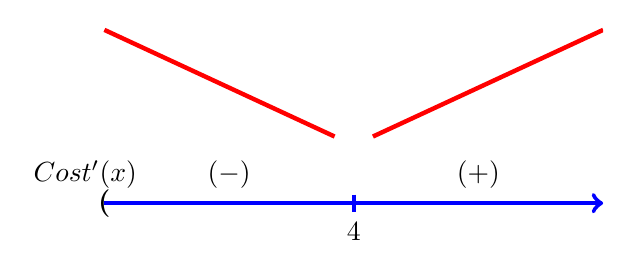
\begin{tikzpicture}
 \begin{axis}[
    	axis x line=none,
	            axis y line=none,
		x label style={anchor=west},
            xlabel={},
            xtick       = {8},
            xticklabels = {$8$},
            y label style={anchor=south},
            ylabel={},
            ytick       = {-6,-4,-2,2,4,6},
            yticklabels = {$-6$,$-4$,$-2$,$2$,$4$,$6$},
            samples     = 320,
            domain      = -2.5:2.5,
            restrict y to domain=-6.5:6.5,
            xmin = 0, xmax = 15,
            ymin = -6.5, ymax = 6.5,
            width=3.5in, height=2.5in,
            grid=none, grid style=solid
          ]
    \addplot[domain= 2:15, blue, ultra thick, mark=none, ->]{0)};
        \addplot[domain= 2:8, red, ultra thick, mark=none, -]{-4/6.5*(x-2)+6)};
         \addplot[domain= 9:15, red, ultra thick, mark=none, -]{4/6.5*(x-15)+6)};
   \draw (1.5,1) node{$\Large Cost^{\prime}(x)$};
   \draw (5.25,1) node{$\Large (-)$};
      \draw (11.75,1) node{$\Large (+)$};
   \draw (2,0) node{ \bf (};
   \draw[ultra thick, blue] (8.5,.3)--(8.5,-.3);
      \draw (8.5,-1) node{$4$};
    \end{axis}
\end{tikzpicture}
\end{center}
Since we have only a single critical number in the domain at $x=4$ and $Cost^{\prime}$ change signs, we know that our Local Minimum is also an Absolute Minimum by the First Derivative Test for Absolute Extrema.\\\\
Lastly we know that one of our dimensions is $x=4cm$. From our volume equation we know that 
\al{
256&=x^2y\\
\frac{256}{x^2}&=y\\
\frac{256}{4^2}&=y\\
16&=y
}
 and the dimensions of our box will be $4cm\times 4cm \times 16cm$.
}


%%%%%%%%%
\newpage%
%%%%%%%%%


\paragraph*{Applied Optimization in Economics}
\begin{itemize}
\item The {\bf unit selling price} is the sales price of a unit of a commodity. The unit selling price of a commodity can vary as the amount of the commodity sold varies, so unit selling price of the $x^{th}$ unit of the commodity can be regarded as a function of $x$, the number of units sold: 
\[p=f(x)\] 
The relationship between $p$ and $x$ is called a {\it demand equation}, the graph of which is called a {\it demand curve}.
\item {\bf Revenue} is the income from the sales of a commodity. If $p(x)$ is the unit selling price of the $x^{th}$ unit of the commodity, then revenue from the sale of $x$ units of the commodity is: \[R(x)=x\cdot p\]
\item {\bf Total cost} is the amount of money that must be spent to produce a commodity. We'll denote the total cost of producing $x$ units of a commodity by $C(x)$.
\item {\bf Profit} is the difference between revenue and total cost:
\[P(x) = R(x) - C(x)\]
\end{itemize}
%
{\exercise}\ltrm{\bf\color{RedOrange}A3} Suppose the unit selling price of a commodity is $p=4-\dfrac1{100}x$ and the total cost of producing a commodity is $C(x)=\dfrac{3}{100}x^2-6x+400$, with $0\leq x\leq 200$ for both.\\
\tasksA{2}{
\task Find \& simplify a revenue function. \\
\sol{\vs{-.15}
 \al{
 R(x)&=x\cdot p\\
R(x) &=x\cdot\left(4-\frac{1}{100}x\right)\\
 R(x)&=4x-\frac{x^2}{100}
 }
}
\task Find \& simplify a profit function.\\
\sol{\vs{-.15}
 \al{
 P(x)&=R(x)-C(x)\\
 &=\left( 4x-\frac{x^2}{100}\right)-\left( \frac{3}{100}x^2-6x+400 \right)\\
 &=4x+6x-\frac{x^2}{100}-\frac{3x^2}{100}-400\\
 &=10x-\frac{4x^2}{100}-400
 }
 }
\task How many units of the commodity should be sold to maximize profit?
}
\sol{
\mpageT{.5}{.5}[\hs{.15}]{\vs{-.2}
\al{
P^{\prime}(x)&=10- \frac{2\cdot 4x^1}{100}-0\\
&=10-\frac{8x}{100}
\intertext{We now check for critical numbers by determining when $P^{\prime}(x)=0$.}
0&\qe10-\frac{8x}{100}\\
\frac{8x}{100}& \qe10\\
8x&\qe1000\\
x&\qe\frac{1000}{8}\\
x&=125
}
}{
We must check if $P^{\prime}(x)=DNE$. We note that $\ds P^{\prime}(x)=10-\frac{8x}{100}$ is a continuous function for all $x$. No values of $x$ will cause any of the following problems: division by $0$, square root of a negative number or log of a negative number or $0$. \\\\Thus the only critical number in our domain is $x=125$. 
}
\newpage
 There are two ways to check to see if $x=125$ is location of Absolute Maximum.
\itemI{
\item {\em Approach 1:}. Since we have a closed interval $[0,200]$, we can check the value of $P(x)$ at the endpoints and at the critical number. 
\itemI{
\item $P(0)=10\cdot 0-\frac{4\cdot 0^2}{100}-400=-400$
\item $P(125)=10\cdot 125-\frac{4\cdot (125)^2}{100}-400=225$
\item $P(200)=10\cdot 200-\frac{4\cdot (200)^2}{100}-400=0$
}
So we do have an Absolute Maximum at $x=125$ units.
\item {\em Approach 2:} Use the First Derivative Test for Absolute Extrema. We create a sign line.
\itemI{
\item We choose a value in $[0,125)$, say $x=0$. $\ds P^{\prime}(0)=10-\frac{8\cdot 0}{100}=10>0$
\item We choose a value in $(125,200]$, say $x=200$. $\ds P^{\prime}(200)=10-\frac{8\cdot 200}{100}=10-16=-6<0$
}  
The sign line below captures this information. We see that we have a local maximum.
   \begin{center}
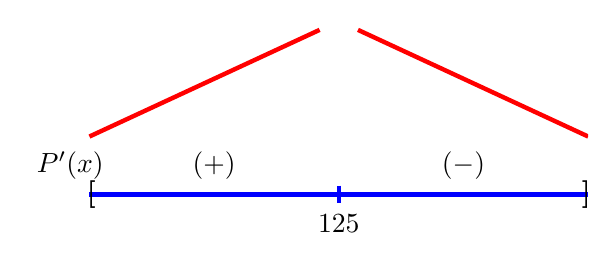
\begin{tikzpicture}
 \begin{axis}[
    	axis x line=none,
	            axis y line=none,
		x label style={anchor=west},
            xlabel={},
            xtick       = {8},
            xticklabels = {$8$},
            y label style={anchor=south},
            ylabel={},
            ytick       = {-6,-4,-2,2,4,6},
            yticklabels = {$-6$,$-4$,$-2$,$2$,$4$,$6$},
            samples     = 320,
            domain      = -2.5:2.5,
            restrict y to domain=-6.5:6.5,
            xmin = 0, xmax = 15,
            ymin = -6.5, ymax = 6.5,
            width=3.5in, height=2.5in,
            grid=none, grid style=solid
          ]
    \addplot[domain= 2:15, blue, ultra thick, mark=none, -]{0)};
        \addplot[domain= 9:15, red, ultra thick, mark=none, -]{-4/6.5*(x-15)+2)};
         \addplot[domain= 2:8, red, ultra thick, mark=none, -]{4/6.5*(x-2)+2)};
   \draw (1.5,1) node{$\Large P^{\prime}(x)$};
   \draw (5.25,1) node{$\Large (+)$};
      \draw (11.75,1) node{$\Large (-)$};
   \draw (2.05,0) node{ \bf [ };
      \draw (14.95,0) node{ \bf ]};
   \draw[ultra thick, blue] (8.5,.3)--(8.5,-.3);
      \draw (8.5,-1) node{$125$};
    \end{axis}
\end{tikzpicture}
\end{center}
}
Since $x=125$ is the only critical number on the domain and because $P^{\prime}$ changes sign, our Local Maximum is also an Absolute Maximum and thus we know selling $x=125$ units will maximize profit.
}



%%%%%%%%%
\newpage%
%%%%%%%%%


{\bf\color{blue}Extra Practice 1.}\ltrm{\bf\color{RedOrange}A3} In economics, the actual cost incurred in producing an additional unit of a certain commodity at a certain level of operation is called the {\bf marginal cost}. Economists often define the marginal cost function to be the derivative of total cost. If the total cost of producing $x$ units of a product is $C(x)=x^2-4x^{3/2}+30$, then find the number of units to produce to minimize the marginal cost function.
\sol{
The Marginal Cost function is $$\ds MC(x)=C^{\prime}(x)=2x-\frac{3}{2}4x^{1/2}+0=2x-6x^{1/2}$$
$x$ is the number of units produced so the domain is $x\geq0$ or $[0,\infty)$. We first find critical numbers.\\
\mpageT{.5}{.5}{\vs{-.2}
\al{
MC(x)&=2x-6x^{1/2}\\
MC^{\prime}(x)&=2-\frac{1}{2}\cdot 6x^{-1/2}\\
&=2-\frac{3}{x^{1/2}}
\intertext{We  check  $MC^{\prime} (x)=0$. }
0&\qe 2-\frac{3}{x^{1/2}}\\
\frac{3}{x^{1/2}}&\qe 2\\
\frac{3}{2}&\qe x^{1/2}\\
\left( \frac{3}{2} \right)^2 & \qe \left( x^{1/2}\right)^2\\
\frac{9}{4}&=x
}
}{
We also check when $MC^{\prime}(x)=DNE$. We note that if $x=0$, $$MC^{\prime}(0)=2-
\frac{3}{0^{1/2}}=DNE$$ Thus we have two critical numbers: $x=0$ and $\ds x=\frac{9}{4}$.\\\\$x=0$ is on the left boundary of our domain $[0,\infty)$. We're would like  to use First Derivative Test for Absolute Extrema. So we create a sign line.
\itemI{
\item We choose a value in $[x,9/4 )$, say $x=1$. $\ds MC^{\prime}(1)=2-\frac{3}{1^{1/2}}=2-3=-1<0$
\item We choose a value in $(9/4,\infty )$, say $x=4$. $\ds MC^{\prime}(4)=2-\frac{3}{4^{1/2}}=2-\frac{3}{2}=\frac{1}{2}>0$
} 
The sign line below captures this information.
}
   \begin{center}
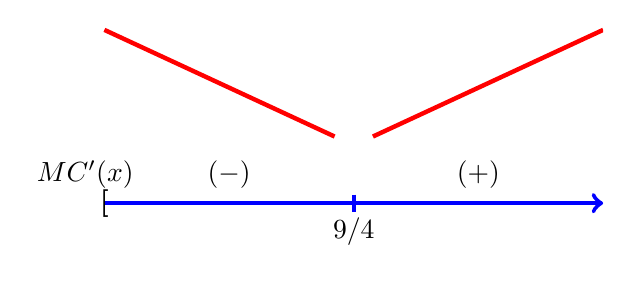
\begin{tikzpicture}
 \begin{axis}[
    	axis x line=none,
	            axis y line=none,
		x label style={anchor=west},
            xlabel={},
            xtick       = {8},
            xticklabels = {$8$},
            y label style={anchor=south},
            ylabel={},
            ytick       = {-6,-4,-2,2,4,6},
            yticklabels = {$-6$,$-4$,$-2$,$2$,$4$,$6$},
            samples     = 320,
            domain      = -2.5:2.5,
            restrict y to domain=-6.5:6.5,
            xmin = 0, xmax = 15,
            ymin = -6.5, ymax = 6.5,
            width=3.5in, height=2.5in,
            grid=none, grid style=solid
          ]
    \addplot[domain= 2:15, blue, ultra thick, mark=none, ->]{0)};
        \addplot[domain= 2:8, red, ultra thick, mark=none, -]{-4/6.5*(x-2)+6)};
         \addplot[domain= 9:15, red, ultra thick, mark=none, -]{4/6.5*(x-15)+6)};
   \draw (1.5,1) node{$\Large MC^{\prime}(x)$};
   \draw (5.25,1) node{$\Large (-)$};
      \draw (11.75,1) node{$\Large (+)$};
   \draw (2,0) node{ \bf [};
   \draw[ultra thick, blue] (8.5,.3)--(8.5,-.3);
      \draw (8.5,-1) node{$9/4$};
    \end{axis}
\end{tikzpicture}
\end{center}
We see that we have a local minimum. We also see that $x=9/4$ is the only place where $MC^{\prime}$ change sign on the domain ($MC^{\prime}(x)$ is undefined at $x=0$ and therefore does not have a sign). Thus by the First Derivative Test for Absolute Extrema, the Local Minimum is also the Absolute Minimum.\\\\
Marginal Cost is minimized when $\ds x=\frac{9}{4}=2.25$ hundred units are sold.
}

%%%%%%%%%
\newpage%
%%%%%%%%%

{\bf\color{blue}Extra Practice 2.}\ltrm{\bf\color{RedOrange}A3} A sheep farmer wishes to construct a rectangular pen enclosing 500 square feet partitioned into two pens using a fence parallel to one of the sides. (See the diagram below.) The fencing for the four outer sides of the pen must be heavy-duty (to keep out predators) and costs \$2 per foot. The interior (subdividing) fence costs \$1 per foot. What are the dimensions of the pen minimizing the cost?\\[0.1in]


\mpageT{.3}{.7}{
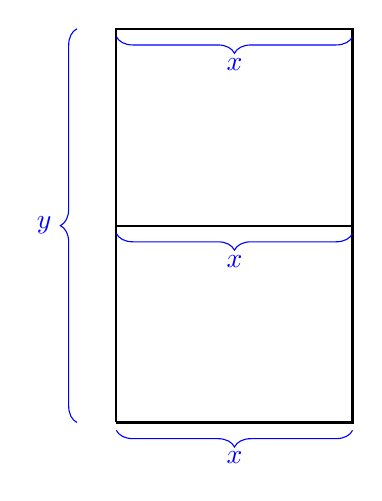
\begin{tikzpicture}
    \draw[thick] (0,0) -- (0,5) -- (3,5) -- (3,0) -- (0,0);
    \draw[thick] (0,2.5) -- (3,2.5);
    \draw [decorate,decoration={brace,amplitude=6pt},xshift=-0.5cm,yshift=0pt, blue]
      (0,0) -- (0,5) node [midway,left,xshift=-.2cm] {\blue{$y$}}; 
        \draw [decorate,decoration={brace,amplitude=6pt},xshift=0cm,yshift=-.1cm, blue]
      (3,0) -- (0,0) node [midway,yshift=-.35cm] {\blue{$x$}}; 
          \draw [decorate,decoration={brace,amplitude=6pt},xshift=0cm,yshift=-.1cm, blue]
      (3,2.5) -- (0,2.5) node [midway,yshift=-.35cm] {\blue{$x$}}; 
                \draw [decorate,decoration={brace,amplitude=6pt},xshift=0cm,yshift=-.1cm, blue]
      (3,5) -- (0,5) node [midway,yshift=-.35cm] {\blue{$x$}}; 
\end{tikzpicture}
}{
\blue{\bf Modeling Phase}
\sol{
\itemI{
\item {\em Quantity to be optimized} We are asked to minimize {\em cost} of a fence when provided information about cost per foot for various types of fencing. 
\item {\em Create relevant variables} We need to define some variables to assist in converting the stated assumptions into mathematical statements.  As in picture on the left, we let $x$ be the width of rectangular pen and $y$ be the length of rectangular pen.
\item {\em Create cost function}. \\ $Cost_{Total}=2\cdot Cost_{side}+ Cost_{top}+Cost_{bottom} +Cost_{interior}$
}
}
}
\blue{
\itemI{
\item For one side, the cost is  is $\$2$ per foot with $y$ feet for each side. Thus $Cost_{side}=2y$.
\item For the top and bottom, the cost is $\$2$ per foot with $x$ feet for each side. Thus $Cost_{top}=2x$ and  $Cost_{bottom}=2x$.
\item For the interior, the cost is $\$1$ per foot with $x$ feet for the interior. Thus $Cost_{interior}=1x=x$
\item Thus 
\al{
Cost_{Total}&=2\cdot Cost_{side}+ Cost_{top}+Cost_{bottom} +Cost_{interior}\\
&=2\cdot(2y)+2x+2x+x\\
Cost_{Total}&=4y+5x
}
\enum{\setItemnumber{4}
\item {\em Find constraint equation} This is a function of both variables $x$ and $y$. In order to minimize this function we need to simplify it to a function of only one variable. We are told that the area of the pen is $500$ square feet.  Thus our constraint equation becomes:
\al{
Area&=x\cdot y\\
500&=xy\\
\frac{500}{x}&=y
}
\item {\em Reduce model function  $Cost_{Total}$ to one variable}.
\al{
Cost_{Total}&=4y+5x\\
&=4\left(\frac{500}{x} \right)+5x\\
C(x)&=\frac{2000}{x}+5x
\intertext{In order to make clear we have a function of only the variable $x$, we have named this cost function $C(x)$.  }
}
\item {\em Identify domain} Since we assume that width is a positive quantity, the domain is $x>0$ or $(0,\infty)$.
}
}
}

\newpage
\blue{\bf Calculus Phase}
\sol{
We need to find critical numbers and test for Absolute Minimum.\\
\mpageT{.5}{.5}{\vs{-.2}
\al{
C(x)&=\frac{2000}{x}+5x\\
&=2000x^{-1}+5x\\
C^{\prime}(x)&=-1\cdot 2000x^{-2}+5\\
C^{\prime}(x)&=-\frac{2000}{x^2}+5\\
C^{\prime}(x)&\qe 0\\
0&\qe -\frac{2000}{x^2}+5\\
\frac{2000}{x^2}&\qe 5\\
\frac{2000}{5}&\qe x^2\\
400&\qe x^2\\
\pm 20&=x
}
}{
We must also check when $C^{\prime}(x)=DNE$. We note that when $x=0$, $$C^{\prime}(0)=-\frac{2000}{0^2}+5=DNE$$ due to division by $0$.\\\\
Thus our critical numbers are t $x=-20,\;0,\;20$. Since $x=20$ is the only critical number in the domain $(0,\infty)$, we will test it to see if we have an Absolute Minimum. We create a sign line.
\itemI{
\item Choose a value in $(0,20)$ say $x=1$. \\$\ds C^{\prime}(1)=-\frac{2000}{1^2}+5=-2000+15=-1995<0$.
\item Choose a value in $(20,\infty)$ say $x=100$. \\$\ds C^{\prime}(100)=-\frac{2000}{(100)^2}+5=-0.2+15=4.8>0$.
}
The sign line below captures this information.
}
   \begin{center}
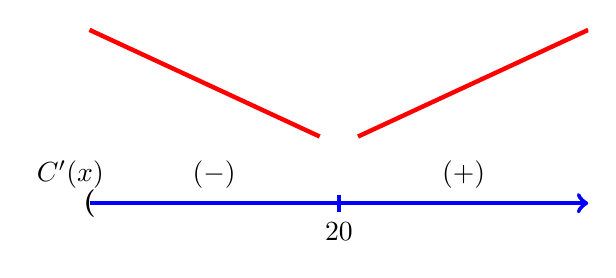
\begin{tikzpicture}
 \begin{axis}[
    	axis x line=none,
	            axis y line=none,
		x label style={anchor=west},
            xlabel={},
            xtick       = {8},
            xticklabels = {$8$},
            y label style={anchor=south},
            ylabel={},
            ytick       = {-6,-4,-2,2,4,6},
            yticklabels = {$-6$,$-4$,$-2$,$2$,$4$,$6$},
            samples     = 320,
            domain      = -2.5:2.5,
            restrict y to domain=-6.5:6.5,
            xmin = 0, xmax = 15,
            ymin = -6.5, ymax = 6.5,
            width=3.5in, height=2.5in,
            grid=none, grid style=solid
          ]
    \addplot[domain= 2:15, blue, ultra thick, mark=none, ->]{0)};
        \addplot[domain= 2:8, red, ultra thick, mark=none, -]{-4/6.5*(x-2)+6)};
         \addplot[domain= 9:15, red, ultra thick, mark=none, -]{4/6.5*(x-15)+6)};
   \draw (1.5,1) node{$\Large C^{\prime}(x)$};
   \draw (5.25,1) node{$\Large (-)$};
      \draw (11.75,1) node{$\Large (+)$};
   \draw (2,0) node{ \bf (};
   \draw[ultra thick, blue] (8.5,.3)--(8.5,-.3);
      \draw (8.5,-1) node{$20$};
    \end{axis}
\end{tikzpicture}
\end{center}
We have a local  minimum at $x=20$. Since this is the only critical number in the domain where $C^{\prime}$ changes sign, the First Derivative Test for Absolute Extrema tells us that the local minimum is also the absolute minimum.  The width of the rectangular pen is $x=20$ ft.  The length of the pen is $\ds y=\frac{500}{20}=25$ ft.
}
\newpage
{\bf\color{blue}Extra Practice 3.}\ltrm{\bf\color{RedOrange}A3} A division of the Chapman Corporation manufactures  a pager. The weekly fixed cost for the division is $\$20,000$ and the variable cost for producing $x$ pagers is $$V(x)=0.000001x^3-0.01x^2+50x$$ dollars. The company realizes a revenue of $$R(x)=-0.02x^2+150x \qquad (0\leq x \leq 7500)$$ from the sale of $x$ pagers per week. Find the level of production that will yield a maximum profit for the manufacturer.
\sol{
Profit = Revenue - Costs.  We are given Revenue as $\ds R(x)=-0.02x^2+150x$. Costs includes both fixed and variable costs. In particular, $C(x)=V(x)+20,000=0.000001x^3-0.01x^2+50x+20,000$. Thus we have
\al{
P(x)&=R(x)-C(x)\\
&=-0.02x^2+150x-\left(0.000001x^3-0.01x^2+50x+20,000 \right)\\
&=-0.02x^2+150x- 0.000001x^3+ 0.01x^2-50x-20,000\\
&=- 0.0001x^3-0.01x^2+100x-20,000\\
P^{\prime}(x)&=-0.000003x^2-0.02x+100-0
}
We need to find critical numbers.  First we check to see when $\ds P^{\prime}(x)=-0.000003x^2-0.02x+100=DNE$. Since this is a quadratic equation, it's defined everywhere and thus we do not encounter the situation when $\ds P^{\prime}(x)=DNE$. We next check when $\ds P^{\prime}(x)=0$. 
\al{
P^{\prime}(x)&=0\\
-0.000003x^2-0.02x+100&=0
\intertext{We use the quadratic formula to find solutions}
x&=\frac{-b \pm \sqrt{b^2-4ac}}{2a}\qquad \text{where $a=-0.000003$, $b=-0.02$, $c=100$}\\
x&=\frac{-(-0.02) \pm \sqrt{(-0.02)^2-4(-0.000003)(100)}}{2(-0.000003)}  \text{ (using technology is ok here)}\\
x&=-10,000 \text{ or } 3,333\frac{1}{3}
}
Since $x=-10,000$ is not in the domain of $0\leq x\leq 7500$, $\ds x=3,333\frac{1}{3}$ is our only critical number. There are two approaches to deciding if we have an absolute max.
\itemI{
\item Approach \#1.  Use the fact that an absolute max must occur at critical numbers or endpoints, we evaluate $P(x)$ at all there points
\itemI{
\item $P(0)=-20,000 $
\item $\ds P(3,333\frac{1}{3})=165,185$
\item $P(7500)=-42,019,000,000$
}
Absolute Max does occur at $\ds x=3,333\frac{1}{3}$ and profit will be $\ds \$165,185$.
\item Approach \#2. Create a sign line for $P^{\prime}$. 
\itemI{
\item Choose a point in the domain to the left of $\ds x=3,333\frac{1}{3}$, say $x=0$.  $\ds P^{\prime}(0)=100>0$
\item Choose a point in the domain to the right of $\ds x=3,333\frac{1}{3}$, say $x=4,000$.  $\ds P^{\prime}(4000)=-28<0$ 
}
The sign line below captures this information.
 \begin{center}
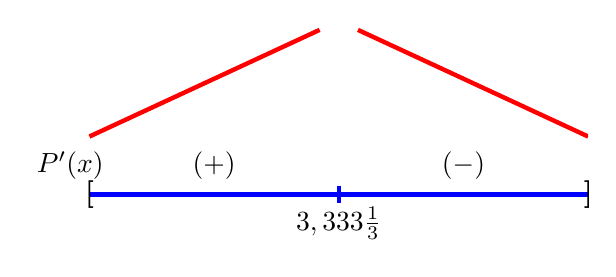
\begin{tikzpicture}
 \begin{axis}[
    	axis x line=none,
	            axis y line=none,
		x label style={anchor=west},
            xlabel={},
            xtick       = {8},
            xticklabels = {$8$},
            y label style={anchor=south},
            ylabel={},
            ytick       = {-6,-4,-2,2,4,6},
            yticklabels = {$-6$,$-4$,$-2$,$2$,$4$,$6$},
            samples     = 320,
            domain      = -2.5:2.5,
            restrict y to domain=-6.5:6.5,
            xmin = 0, xmax = 15,
            ymin = -6.5, ymax = 6.5,
            width=3.5in, height=2.5in,
            grid=none, grid style=solid
          ]
    \addplot[domain= 2:15, blue, ultra thick, mark=none]{0)};
        \addplot[domain= 9:15, red, ultra thick, mark=none, -]{-4/6.5*(x-15)+2)};
         \addplot[domain= 2:8, red, ultra thick, mark=none, -]{4/6.5*(x-2)+2)};
   \draw (1.5,1) node{$\Large P^{\prime}(x)$};
   \draw (5.25,1) node{$\Large (+)$};
      \draw (11.75,1) node{$\Large (-)$};
   \draw (2,0) node{ \bf [};
      \draw (15,0) node{ \bf ]};
   \draw[ultra thick, blue] (8.5,.3)--(8.5,-.3);
      \draw (8.5,-1) node{$3,333\frac{1}{3}$};
    \end{axis}
\end{tikzpicture}
\end{center}
}
Thus we have a local max at $\ds x=3,333\frac{1}{3}$. The First Derivative Test for Local Extrema tells us that since we have only one critical number where  $P^{\prime}(x)$ changes sign, the Local Max is also the Absolute Max.
}
\end{document}
